\chapter{Modulares Eingabesystem}
\section{Vision}
Das Eingabesystem verfolgt die Vision eines flexiblen und erweiterbaren Steuerungssystems, das sich an die individuellen Bedürfnisse der Benutzer anpasst. Im Zentrum dieser Vision steht ein Hauptmodul, das als Mikrocontroller-Einheit dient und über eine USB-Schnittstelle mit einem Computer verbunden wird. Dieses Hauptmodul koordiniert die Kommunikation und Funktionalität der angeschlossenen Module.
\\
\\
Die Module des Systems, wie das Tastatur-Modul mit einer 4x4-Tastenmatrix oder das Audio-Modul mit Potentiometern und Pegelstellern, sind frei kombinierbar und können je nach Anwendungsfall hinzugefügt oder entfernt werden. Dies ermöglicht eine maßgeschneiderte Konfiguration für unterschiedliche Aufgaben wie Textverarbeitung, Bildbearbeitung, Audiobearbeitung oder Gaming.
\\
\\
Die folgende Abbildung gewährt einen Überblick über das Eingabesystem:
\begin{figure}[H]
    \centering    
    \fbox{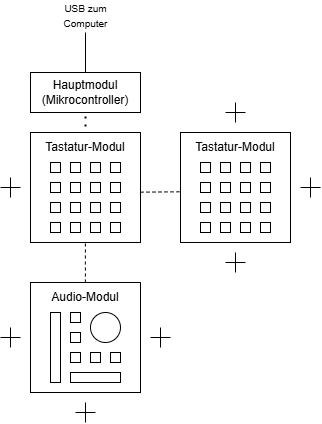
\includegraphics[width=.75\textwidth]{Bilder/bu_vision.png}}
    \caption{Vereinfachte Darstellung des Eingabesystems}
    \label{A3TPHP}
\end{figure}
\noindent Die gestrichelten Linien stellen eine bereits hergestellte Verbindung zwischen den Modulen dar, wobei die \glqq Plus\grqq{} Symbole einen weiteren möglichen Modulanschluss darstellen. Die Module werden untereinander durch die Verwendung von Pogo-Pin-Steckern verbunden.
\subsection{Steckverbindung}
Zwischen den Modulen werden Daten und Spannungsversorgung über eine 4 Pin-Verbindung realisiert. Diese sind VCC (Spannungsversorgung), Data + (Datenbus), Data - (invertierter Datenbus) und GND (Masse). Da der Benutzer die Möglichkeit haben soll, jedes Modul an jede Seite eines anderen anstecken zu können, werden pro Seite zwei 2-Pin Pogo Stecker verwendet, ein 2-Pin Male und ein 2-Pin Female Stecker. Dadurch kann durch kluge Positionierung jede Seite eines Moduls mit jeder Seite eines anderen verbunden werden.
\begin{figure}[H]
    \centering    
    \fbox{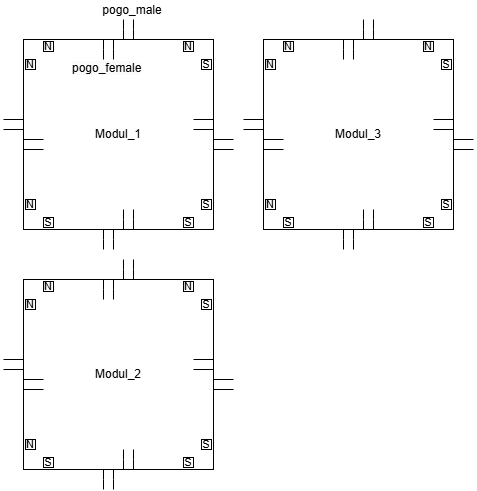
\includegraphics[width=.75\textwidth]{Bilder/bu_pogoverbindung.png}}
    \caption{Pogo verbindung}
    \label{pogo_verbindung}
\end{figure}
 \noindent Abbildung \ref{pogo_verbindung} zeigt, dass die Steckverbindungen jede beliebige Anordnung der Module zulassen.